
\part[Estrutura de dados n-dimensionais homogêneas]
{Estrutura de dados n-dimensionais homogêneas}


\chapter[Vetores]
{Vetores}



\section{Resumo}

Vetores são um tipo de estrutura que podem armazenar um tamanho fixo de elementos do mesmo tamanho e mesmo tipo, alocados em memória contígua. Utiliza-se vetores como um tipo de lista unidimensional, acessada através de índices.


%\begin{chapreferences}{1.}
%\bibliography{playcb}
%\bibliographystyle{plain}
%\nocite{cbook}
%\nocite{sb6}
%\nocite{glfw}
%\nocite{cppbook}

%\end{chapreferences}

% \begin{chapreferences}{1}

% \bibitem{sb6}
% {\em OpenGL SuperBible}.
% \newblock Pearson Education Inc, 6 edition, 2014.

% \bibitem{glfw}
% Marcus Geelnard and Camilla Berglund.
% \newblock {\em GLFW - Reference guide}, 2010.
% \newblock API version 2.7.

% \bibitem{cbook}
% Brian~W. Kernighan and Dennis~M. Ritchie.
% \newblock {\em The C Programming Language}.
% \newblock 1989.

% \bibitem{cppbook}
% Stanley~B. Lippman, Josés Lajoile, and Barbara Moo.
% \newblock {\em C++ Primer}.
% \newblock 2013.
% \end{chapreferences}


\section{Criando um gráfico}
\begin{figure}[ht]
  \centerline{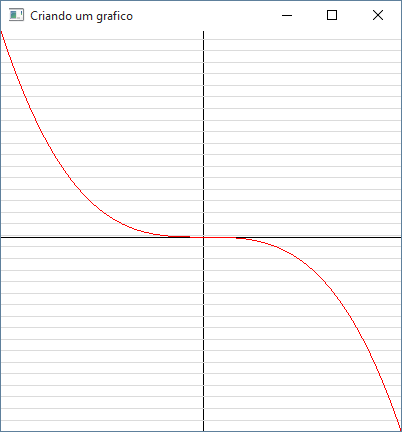
\includegraphics[width=.5\textwidth]{img/cap2_ex8.png}}
  \caption{Gráfico do polinômio $-x^3$}
  \label{fig:cap02_ex1}
\end{figure}
Esta prática mostra como construir um gráfico a partir de um vetor de Pontos. Cada posição em \emph{y} de cada ponto é calculada dentro do loop. Por padrão, os limites da janela de exibição da playCB vão de -100 à 100, entretanto, os valores em \emph{y} nesta função variam de $-125.000$ até $125.000$, tendo a necessidade de mudar o limite de exibição com a função \emph{MudaLimitesJanela(125000)}.
\lstinputlisting[caption=Código fonte de polinômio, style=customc, label=lst:cap2_ex8]{src/ex8_grafico.cpp}

\chapter[Matrizes]
{Matrizes}



\section{Resumo}

Assim como vetores, matrizes são um tipo de estrutura que armazena dados de mesmo tamanho e mesmo tipo, mas são utilizadas de maneira n-dimensional. O modo mais comum de utilizar matriz é usando-a na forma bidimensional, onde os dados são tratados como se estivessem numa tabela, com linhas e colunas.


%\begin{chapreferences}{1.}
%\bibliography{playcb}
%\bibliographystyle{plain}
%\nocite{cbook}
%\nocite{sb6}
%\nocite{glfw}
%\nocite{cppbook}

%\end{chapreferences}

% \begin{chapreferences}{1}

% \bibitem{sb6}
% {\em OpenGL SuperBible}.
% \newblock Pearson Education Inc, 6 edition, 2014.

% \bibitem{glfw}
% Marcus Geelnard and Camilla Berglund.
% \newblock {\em GLFW - Reference guide}, 2010.
% \newblock API version 2.7.

% \bibitem{cbook}
% Brian~W. Kernighan and Dennis~M. Ritchie.
% \newblock {\em The C Programming Language}.
% \newblock 1989.

% \bibitem{cppbook}
% Stanley~B. Lippman, Josés Lajoile, and Barbara Moo.
% \newblock {\em C++ Primer}.
% \newblock 2013.
% \end{chapreferences}


\section{Criando um gráfico}
\begin{figure}[ht]
  \centerline{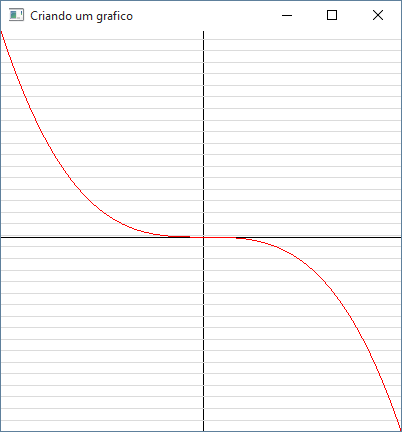
\includegraphics[width=.5\textwidth]{img/cap2_ex8.png}}
  \caption{Gráfico do polinômio $-x^3$}
  \label{fig:cap02_ex1}
\end{figure}
Esta prática mostra como construir um gráfico a partir de um vetor de Pontos. Cada posição em \emph{y} de cada ponto é calculada dentro do loop. Por padrão, os limites da janela de exibição da playCB vão de -100 à 100, entretanto, os valores em \emph{y} nesta função variam de $-125.000$ até $125.000$, tendo a necessidade de mudar o limite de exibição com a função \emph{MudaLimitesJanela(125000)}.
\lstinputlisting[caption=Código fonte de polinômio, style=customc, label=lst:cap2_ex8]{src/ex8_grafico.cpp}
